% Created 2023-04-17 Mon 02:36
% Intended LaTeX compiler: pdflatex
\documentclass[twocolumn]{article}
\usepackage[utf8]{inputenc}
\usepackage[T1]{fontenc}
\usepackage{graphicx}
\usepackage{longtable}
\usepackage{wrapfig}
\usepackage{rotating}
\usepackage[normalem]{ulem}
\usepackage{amsmath}
\usepackage{amssymb}
\usepackage{capt-of}
\usepackage{hyperref}
\usepackage{balance}
\usepackage{graphics}
\usepackage{txfonts}
\usepackage{times}
\usepackage{color}
\usepackage{textcomp}
\usepackage{booktabs}
\usepackage{todonotes}
\usepackage{float}
\usepackage{url}
\usepackage{titling}
\usepackage[left=3cm,right=2cm,top=2.5cm,bottom=2cm]{geometry}
\usepackage[british]{babel}
\usepackage{sectsty}
\sectionfont{\Large}
\subsectionfont{\large}
\subsubsectionfont{\large}
\paragraphfont{\normalsize}
\setlength{\parindent}{0em}
\setlength{\parskip}{1em}
\setlength{\columnsep}{2em}
\setlength{\droptitle}{-5em}
\makeatletter
\def\url@leostyle{%
\@ifundefined{selectfont}{\def\UrlFont{\sf}}{\def\UrlFont{\small\bf\ttfamily}}}
\makeatother
\urlstyle{leo}
\usepackage[
%backend=biber,
natbib=true,
style=numeric,
sorting=none
]{biblatex}
\addbibresource{/home/struan/Documents/University/Dissertation/library.bib}
\addbibresource{/home/struan/Sync/library.bib}
\author{Struan Robertson \\ BSc (Hons) Applied Computing}
\date{May 2023}
\title{Terrain Model Processing with Machine Learning}
\hypersetup{
 pdfauthor={Struan Robertson \\ BSc (Hons) Applied Computing},
 pdftitle={Terrain Model Processing with Machine Learning},
 pdfkeywords={},
 pdfsubject={},
 pdfcreator={Emacs 28.2 (Org mode 9.6.1)}, 
 pdflang={English}}
\begin{document}

\maketitle
\begin{abstract}

With the launch of the lunar orbiter laser altimeter (LOLA) on NASA's lunar reconnaissance orbiter (LRO), a large amount of high-resolution digital elevation maps (DEMs) have been constructed, providing a precise topographical model of the moons surface.
These DEMs are prone to voids containing no data, making the map less reliable for scientific purposes and future moon missions.
This paper uses a machine learning model to allow for the technique of image inpainting to be used with lunar DEMs.
Image inpainting uses pixel data from an image to generate missing data to fill a void.
DEMs can be thought of mathematically as identical to a single channel (greyscale) image, a two-dimensional array with "pixel" values corresponding to height, and so the technique of image inpainting can be easily applied to DEMs.
A Generative Adversarial Network (GAN) based on a fully convolutional architecture was used for the inpainting.


\end{abstract}

\section{Introduction}
\label{sec:org8900d0b}

Sensory data from the Lunar Orbiter Laser Altimeter (LOLA) and Lunar Reconnaissance Orbiter Camera (LROC) has been used for the construction of Lunar digital elevation models (DEMs) since the launch of the Lunar Reconnaissance Orbiter (LRO) in 2009.
LRO has several primary objectives as part of a series of robotic missions that aim to pave the way for a permanent human presence on the Moon, including determining the global topography of the lunar surface at meter-scale resolution.
Topographical data from LOLA and LROC will be used to facilitate the selection of future landing sites, so accuracy and completeness are essential.
\autocite{chinLunarReconnaissanceOrbiter2007}

The LRO is in a polar orbit around the moon, scanning the surface in swathes 50 to 60m wide, with an average separation ranging between 1.2km and 200m depending on the position of LRO in orbit.
LOLA uses a laser altimeter to measure the distance from LRO to the lunar surface at 5 different spots simultaneously, providing DEMs ranging from \textasciitilde{}30m resolution at the equator to \textasciitilde{}5m resolution at the poles. \autocite{smithLunarOrbiterLaser2010}.
LROC uses two narrow-angle cameras (NACs) to collect stereo observations at a resolution of 0.5 to 1.5 m per pixel.
These high resolution images can be used to generate high resolution (\textasciitilde{}5m at the equator) DEMS, referred to as NAC DEMs \autocite{tranGeneratingDigitalTerrain2010}.

Both LOLA and NAC dems are prone to no-data voids resulting from shadowed regions (NAC) or terrain features blocking the return of the laser altimeter (LOLA).
As the LRO has a polar orbit, data is recorded in strips, which must be joined together to create larger DEMs. These strips are not immediately adjacent to each other, resulting in a no-data void in-between.
Reconstructing these no-data voids is non-trivial, with Park and Choi \autocite{parkNeuralProcessApproach2021}  noting the following challenges:
\begin{itemize}
\item NAC DEMs require high-resolution reconstruction methodology
\item NAC DEMs are large and high-resolution area maps, thus a scalable approach should be applied
\item The reconstruction algorithm must be reliable since it can affect related lunar studies or exploration missions
\end{itemize}

Traditional algorithmic methods for correcting no-data voids within DEMs include inverse distance weight method (IDW), local polynomial interpolation method (LPI), spline with tension method (ST) and other algorithms to interpolate the elevation sampling points. Interpolation methods use the neighboring elevation values for void infilling, thus performance is directly proportional to the size of the void.
Voids of any significant size result in interpolation methods returning inaccurate reconstruction results.  \autocite{reuterEvaluationVoidFilling2007}

Within the field of computer vision, the problem of image inpainting fundamentally seeks to solve the same issue as DEM void infilling; a 2-dimensional grid of points with an area of no data which must be inferred from surrounding points.
RGB images contain three channels whereas a DEM contains only one, however inpainting techniques process each channel independently and then combine the results, so inpainting a DEM is functionally identical to inpainting a greyscale image.
Generative adversarial networks (GANs)\autocite{goodfellowGenerativeAdversarialNetworks2020} are a deep learning generative model that when constructed with deep convolutional neural networks\autocite{krizhevskyImageNetClassificationDeep2017} have been shown to have excellent performance in image inpainting\autocite{pathakContextEncodersFeature2016,yuGenerativeImageInpainting2018} and have been successfully applied to the task of DEM void infilling\autocite{gavriilVoidFillingDigital2019,zhangVoidFillingBased2020,qiuVoidFillingDigital2019}.

This papers implements a GAN inpainting network based on the structure described by Yu \emph{et al.}\autocite{yuGenerativeImageInpainting2018} and shows it to effectively pass the first two challenges set forward by Park and Choi\autocite{parkNeuralProcessApproach2021}.
The final challenge of DEM reliability may be passed by this network, however this is difficult to test as GANs excel at infilling \emph{plausible} data, yet the \emph{accuracy} of this data may not be necessarily sufficient.


\section{Background}
\label{sec:org30a68e1}
\subsection{Digital Elevation Maps}
\label{sec:org0a54a20}

Digital elevation maps (DEMs) are digital representations of terrain elevation (Figure \ref{fig:apollo_17}).
A DEM consists of a grid of cells, where each cell represents a specific area of terrain and contains the elevation value of the ground at this location.
The cells of a DEM can also be described as pixels, as they represent a discrete location in a raster grid.
DEM gridsize refers to the size of cells and can be thought of as the resolution of the DEM.
Gridsize can vary depending on the source of data and the intended application, with common grid sizes ranging from a few meters to several kilometers.

\begin{figure}[htbp]
\centering
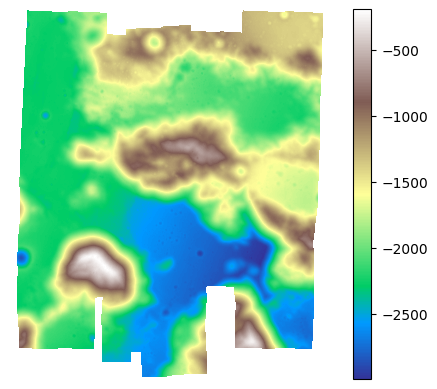
\includegraphics[width=.9\linewidth]{images/apollo_17.png}
\caption{\label{fig:apollo_17}Shaded DEM of Apollo 17 landing site in Taurus-Littrow Valley}
\end{figure}

\begin{figure}[htbp]
\centering
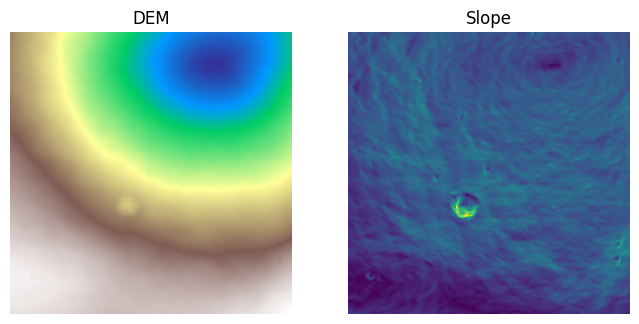
\includegraphics[width=.9\linewidth]{images/dem_and_slope.png}
\caption{\label{fig:dem_and_slope}Section of DEM with computed slope}
\end{figure}

The slope of a DEM refers to the steepness of terrain at each location in the map (Figure \ref{fig:dem_and_slope})
Slope is calculated by traversing a 3 x 3 window (Figure \ref{fig:window}) over the DEM\autocite{qiuVoidFillingDigital2019}.
The slope value at the central pixel \emph{e} can be calculated by using the algorithm proposed by Horn \emph{et al.}\autocite{hornHillShadingReflectance1981} :
\begin{align}
Slope &= arctan\sqrt{Slope^2_{we} + Slope^2_{sn}}, \\
Slope_{we} &= \frac{(e_8 + 2e_1 + e_5) - (e_7 + 2e_3 + e_6)}{8 \times Gridsize}, \\
Slope_{sn} &= \frac{(e_7 + 2e_4 + e_8) - (e_6 + 2e_2 + e_5)}{8 \times Gridsize},
\end{align}

\begin{figure}[htbp]
\centering
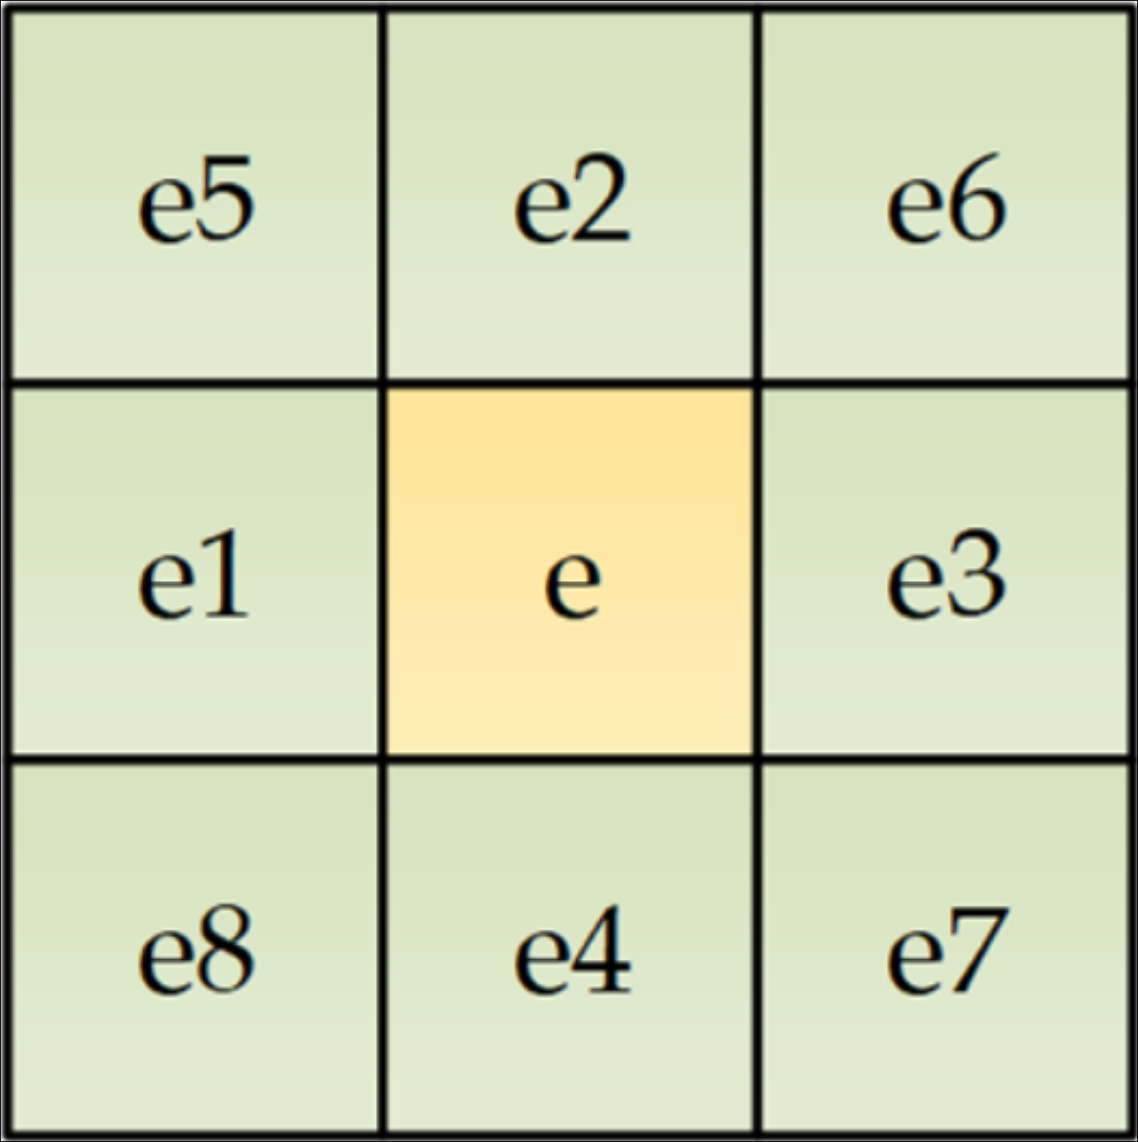
\includegraphics[width=4cm]{images/window.png}
\caption{\label{fig:window}The 3x3 moving window\autocite{qiuVoidFillingDigital2019}}
\end{figure}

The most common data format for the storage of DEMs is GeoTiff.
A GeoTiff is a type of TIFF (Tagged Image File Format) that with the raw DEM raster data also stores spatial metadata such as pixel resolution (gridsize).
Lunar DEMs are also commonly stored in NASA's PDS (Planetary Data System) archival formats PDS3 and PDS4.
PDS is used to archive multiple kinds of data from planetary science missions, not just DEMs.
Older missions (pre 2011) are typically archived in PDS3, with post 2011 missions using PDS4.
Although stored differently, the raster data in PDS files and GeoTiffs is identical.

The issue of no-data voids is not limited to lunar DEMs, as DEMs are typically constructed using remote sensing technology which is prone to the same errors.

\subsection{Deep Neural Networks}
\label{sec:orge1d5366}

Neural networks are a type of machine learning algorithm that is loosely modeled after the structure and function of biological brains, consisting of multiple artificial neurons\autocite{grossiIntroductionArtificialNeural2008}.
A neuron can hold any value, however in most neural networks this value is restricted between 0 and 1 or -1 and 1.
The value a neuron holds is referred to as its activation.
When data is passing forwards through a network, each neuron has an activation determined by the input data.
In a fully connected network, these neurons are arranged into layers, with every neuron in a layer connected to every neuron in the previous layer (Figure \ref{fig:neural_network}) .
The first layer is the input layer, the last the output layer and the layers in-between are hidden layers.
In image processing tasks, such as image inpainting, the neurons in the input layer correspond to the pixels of the input image.
The layered structure of the neural network is highly efficient as it allows the network to break down complex problems into smaller steps.

\begin{figure}[htbp]
\centering
\includegraphics[width=.9\linewidth]{images/neural_network.png}
\caption{\label{fig:neural_network}Simple feedforward artifical neural network\autocite{ArtificialNeuralNetwork2023}}
\end{figure}

Each connection between neurons in different layers has an associated weight.
This weight is an indication of how the neuron in the second layer is correlated to the neuron in the first.
A positive weight indicates that when the first neuron has a high activation so should the second, and a negative weight the inverse.
Each neuron also holds a value called a bias, which can be thought of as the minimum weighted sum for the neuron to activate.
To compute the activation of a second layer neuron, take the sum of the activations of the first layer neurons multiplied with their weights and add the bias (Equation \ref{eqn:activation}).
The activation can be any number, however to normalise the signal between a range and add non-linearity to the network the activation is passed through an activation function.

ReLU (Rectified Linear Unit) is an activation function which can introduce sparsity into the network, meaning only a subset of neurons will be activated for any given input.
The constant gradient of ReLU when the gradient is positive improves the stability of gradients in the network, making vanishing gradients less likely than other activation functions, such as sigmoid.
ReLU also introduces sparsity in the activations since it outputs zero for negative input values.
Whilst this can simplify the network and reduce computational complexity, it can also lead to the "dying ReLU" problem, where some neurons in the network stop contributing to the output due to always receiving negative input values and having an output of zero.
The ELU activation function (Figure \ref{fig:ELU}) becomes smooth slowly until its output equals \(-\alpha\) for negative inputs, ensuring all neurons in the network can contribute to the output even if their inputs are negative.
This can improve the performance of the network when dealing with noisy or outlier data, which is very common in DEMs.
For this reason ELU is the most common activation function in the network described by this paper.
Other activation functions used are Leaky ReLU and Tanh.
Leaky ReLU also addresses the dying ReLU problem, however instead of a smooth curve to \(-\alpha\), negative values have a small constant negative slope equal to \(\alpha\) (usually 0.1).
Leaky ReLU is used in the discriminator of this the network described by this paper as it allows the activation to be infinitely small.
In generative networks such as the generator, this can lead to vanishing gradients, however in classifier networks such as the discriminator it is important for it to be able to learn negative associations.
The Tanh activation function compresses all activations to between -1 and 1, and so is used as the final layer in generative networks to produce output data of the same range as the input data.

\begin{equation}
\label{eqn:activation}
a^{(1)}_0 = ELU(w_{0,0}a^{(0)}_0 + w_{0,1}a^{(0)}_1 + \cdots + w_{0,n}a^{(0)}_n + b_0)
\end{equation}

\begin{figure}[htbp]
\centering
\includegraphics[width=.9\linewidth]{images/ELU.png}
\caption{\label{fig:ELU}ELU activation function}
\end{figure}


As the equations are linear, to efficiently compute the activation of every neuron in a forward layer, the equations can be stacked into matrices\autocite{3Blue1BrownWhatNeural} :
\begin{equation}
\begin{bmatrix} a^{(1)}_0 \\ a^{(1)}_1 \\ \vdots \\ a_n^{(1)} \end{bmatrix} = ELU \left( \begin{bmatrix}w_{0,0} & w_{0,1} & \dots & w_{0,n} \\ w_{1,0} & w_{1,1} & \dots & w_{1,n} \\ \vdots & \vdots & \ddots & \vdots \\ w_{k,0} & w_{k,1} & \dots & w_{k,n} \end{bmatrix} \begin{bmatrix} a_0^{(0)} \\ a_1^{(0)} \\ \vdots \\ a_n^{(0)} \end{bmatrix} + \begin{bmatrix} b_0 \\ b_1 \\ \vdots \\ b_n \end{bmatrix} \right)
\end{equation}

A cost function such as Mean Squared Error (MSE) is used to measure how well the network is performing.
As the network is itself a function, the cost function is a function which takes all the weights and biases of the network as inputs and returns a value describing how well these weights and biases perform.
A neural network is trained with the following steps.
Input data is propagated forwards through the network layer by layer.
The cost function is then evaluated using the predicted output and the actual output, with the error between the two values calculated.
The error is then backpropagated through the network, layer by layer, starting from the output layer.
The desired output of the output layer is known, so by working backwards layer by layer the activations of each neuron that would have resulted in the desired output can be calculated.
The error at each layer is used to calculate the gradient of the cost function with respect to the weights of that layer\autocite{leTutorialDeepLearning2015}.
The weights and biases of the network are updated using the gradients calculated during backpropagation by using an optimisation algorithm such as stochastic gradient descent (SGD)\autocite{ruderOverviewGradientDescent2016}, which adjusts the weights and biases in a way that takes a step down the gradient towards a local minimum of the cost function; with the steeper the gradient the greater the step taken.
The network can become stuck in a local minimum, as it is impossible to know what the true minimum is, only the downwards direction is known.
An analogy for this would be rolling a ball down a hill.

As calculating the gradient for the entire dataset is very computationally difficult, the data is batched, with the cost function calculated for each example in a batch and then averaged to get a single cost value for the batch - which is then backpropagated.
This average is important, as the ideal adjustment to weights and biases will be different for each piece of input data, so by averaging the cost function of each a generalised value is reached.
An epoch is the entire set of training data. It normally takes multiple epochs of training data for the network to converge at a set of weights that minimise the cost function.

A deep neural network is functionally the same, however it involves more hidden layers than the classical network described above.

\textbf{Batch Normalisation} TODO

\subsubsection{Convolutional Neural Networks}
\label{sec:org72f4b33}

\begin{figure}[htbp]
\centering
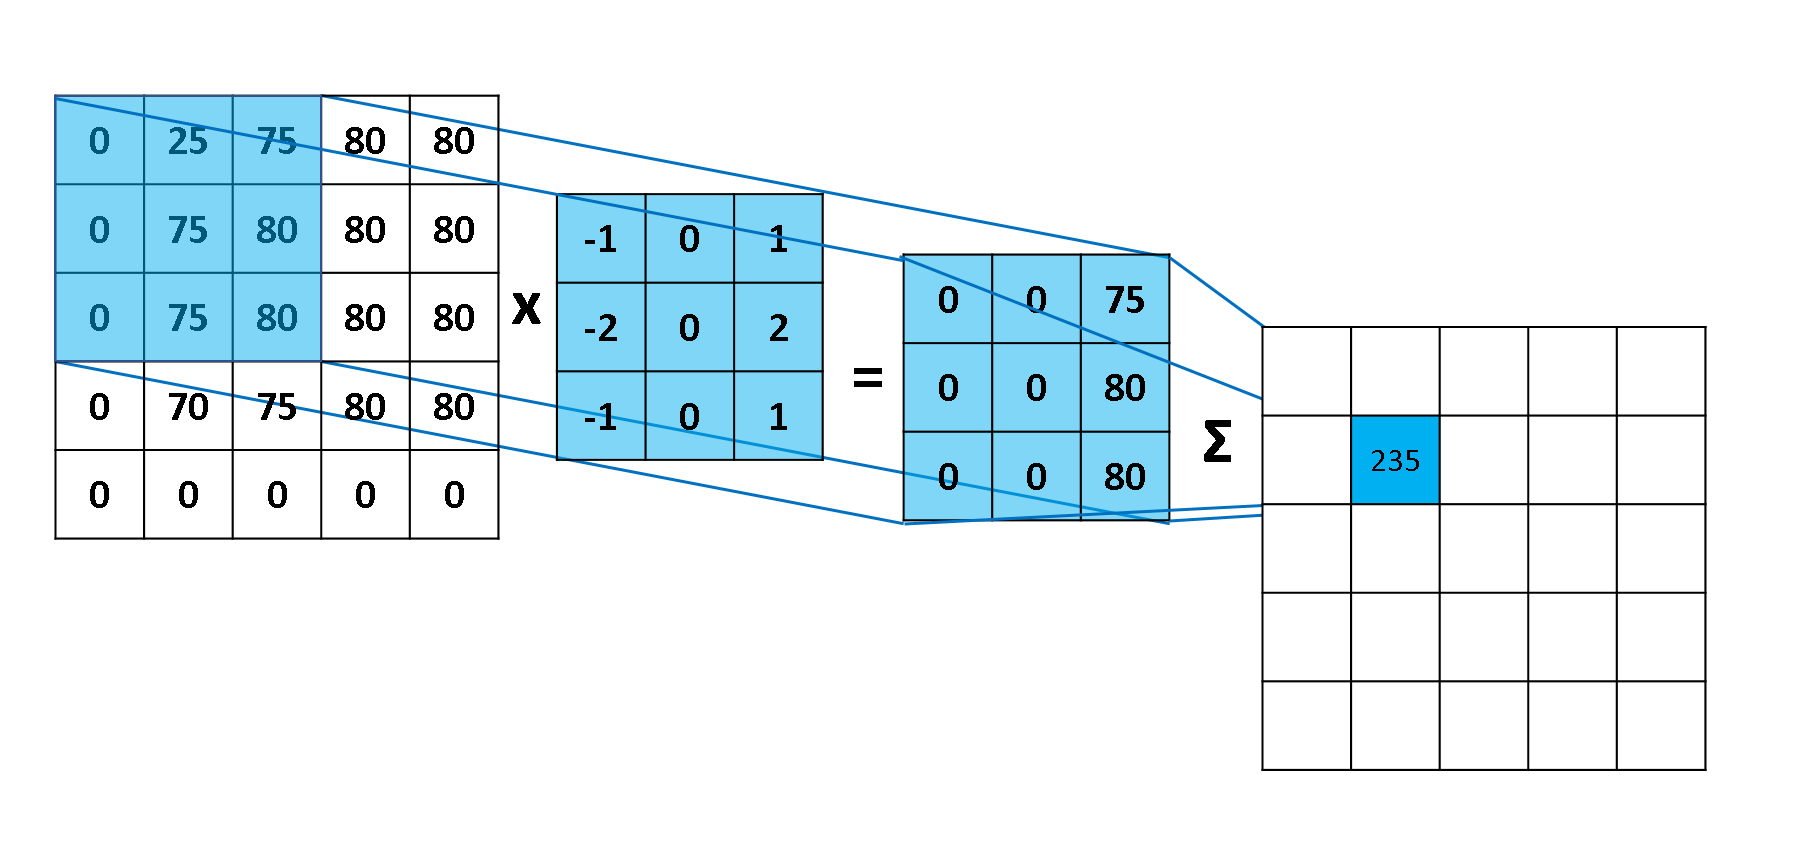
\includegraphics[width=.9\linewidth]{images/convolution.png}
\caption{\label{fig:convolution}Convolution step\autocite{ConvolutionalNeuralNetworks}}
\end{figure}

A convolutional neural network (CNN) is comprised of layers of 2D convolutions.
These layers consist of filters which themselves are comprised of kernels, small matrices with learned weights as values\autocite{osheaIntroductionConvolutionalNeural2015}.
Filters have a kernel for each input channel to the layer, with each kernel moving accross the channel and performing an elementwise multiplication with the part of the input it is currently on (Figure \ref{fig:convolution}).
The results of all kernels in a filter are summed into a single output pixel, meaning that each filter produces one output channel.
The stride of the layer determines how far the filter moves over the data every convolution, therefore a stride greater than one reduces the spatial dimensions by a factor of the stride size\autocite{dumoulinGuideConvolutionArithmetic2018}.
The inverse is also true, a sub-pixel stride of less than one increases the spatial dimensions, however this can lead to checkerboard artifacts where kernels overlap so a more appropriate technique is to interpolate the image into a larger size and then convolve over it, referred to as a resize-convolution\autocite{odenaDeconvolutionCheckerboardArtifacts2016}\autocite{aitkenCheckerboardArtifactFree2017}

\begin{figure}[htbp]
\centering
\includegraphics[width=.9\linewidth]{images/convolution_filter.png}
\caption{\label{fig:convolution_filter}Visualised convolution filters, with increasing complexity of features extracted\autocite{graetzHowVisualizeConvolutional2019}}
\end{figure}

Each kernel is unique, with the values of the matrix being the weights learned by through training.
Filters have a bias, which gets added to all values in the output data.
By using multiple filters with a stride greater than 1, the number of output channels can be increased whilst the spatial dimensions of the data is decreased.
This is a fundamental pattern in a CNN, as it allows for kernels to learn to extract features.
By reducing the spatial dimensions of the image, earlier layers extract low level features which get combined by following layers (Figure \ref{fig:convolution_filter}).
The compression of the input data also allows for later kernels to extract patterns from an area much larger than their kernel size .
Dilated convolutions expand the kernel by inserting holes between its elements, allowing the kernel to cover a larger area than its size\autocite{dumoulinGuideConvolutionArithmetic2018}.


\begin{figure}[htbp]
\centering
\includegraphics[width=.9\linewidth]{images/autoencoder.png}
\caption{\label{fig:autoencoder}Simplified diagram of an autoencoder\autocite{birlaAutoencoders2019}}
\end{figure}

\textbf{Autoencoders}

Autoencoders construct an encoder and decoder out of convolutional layers, using the change in channel number and spatial dimensions to learn to deconstruct then reconstruction data (Figure \ref{fig:autoencoder}).
The encoder is trained to reduce the spatial dimensions of the input data whilst increasing the number of channels.
The latent space is the result of this encoding, a lower-dimensional compressed representation of the data.
In a trained network, the latent space captures the most important features and patterns of the input data in a compact and efficient way\autocite{michelucciIntroductionAutoencoders2022}.
This representation is generalised, two different craters would be represented as craters, even if they had visual differences.
Autoencoders are useful for image inpainting as the latent space more clearly demonstrates the missing parts of features.
Dilated convolutions are especially effective in latent space, as the kernel acts over a larger area of the already compressed data for little computational cost, allowing it to learn complex and large features.
The decoder is trained to translate the latent space back into the inpainted image.
A famous use of autoencoders is in early "deepfake" networks, which are designed to swap faces in images.
In a deepfake network, separate autoencoders are trained for the two faces.
By swapping the decoder from one autoencoder into another, the autoencoder encodes properties (such face angle) for one face, however decodes the image with the other face.


\subsubsection{Generative Adversarial Networks}
\label{sec:org56b395e}
Generative adversarial networks (GANs)\autocite{goodfellowGenerativeAdversarialNetworks2020} are a machine learning framework based on game theory.
They are constructed from two opposing networks, a generator and a discriminator.
The generator learns to generate fake data and attempts to trick the discriminator, which learns to distinguish between real and fake samples.
The adversarial loss between the competing networks is able to catch errors which would be overlooked by other loss functions, such as mean squared error\autocite{lotterUnsupervisedLearningVisual2016}.

A difficult challenge of training GANs is keeping the training of both generator and discriminator balanced.
If one network becomes substantially better than the other, the gradient for the better network will explode and the other networks gradient will vanish.
Wasserstein GANs\autocite{arjovskyWassersteinGenerativeAdversarial2017} improve this situation by using the Wasserstein-1 distance to measure discrepancy between real and generated data distributions.
The Wasserstein-1 distance is a measure of how much effort it would take to move one probability density into another, which is continuous in nature, leading to more stable gradients.
To further improve the stability of the network, a gradient penalty can be applied to the network to ensure that both generator and discriminator train at similar rates\autocite{gulrajaniImprovedTrainingWasserstein2017}.
If one trains faster than the other, the gradient descent is penalised to allow the other to close the gap.

A GAN containing only convolutional layers is referred to as a deep convolutional GAN\autocite{radfordUnsupervisedRepresentationLearning2016}.
This simplification of the network is more computationally efficient than the GAN first proposed by Goodfellow et al.\autocite{goodfellowGenerativeAdversarialNetworks2020}, whilst allowing for deeper models and increased image resolution.
GANs typically use encoders and decoders, as novel data can be hallucinated in the latent space and then decoded to the output.
The addition of dilated convolutions\autocite{yuMultiScaleContextAggregation2016} as four layers in the latent space adds an enhanced receptive field, allowing for improved feature learning.

GAN training is unsupervised, meaning that it the training data set does not need to be labeled.
This is because data is known to be real or generated, and so the loss function can operate independently.
As training neural networks requires large amounts of data, unsupervised training requires far less human effort to achieve.
GANs are well suited for the task of void infilling, as the adversarial loss results in the generator being trained to generate the accurate DEMs, without the need of manually labeling voids locations.

\begin{figure}[htbp]
\centering
\includegraphics[width=.9\linewidth]{images/contextual_attention.png}
\caption{\label{fig:contextual_attention}Contextual attention focusing network on cat \autocite{zhangAgileAmuletRealTime2018}}
\end{figure}

\textbf{Contextual Attention}

Image features are extracted in convolutional neural networks with local kernels layer by layer.
This locality reduces the kernels effectiveness at borrowing from distant spatial locations; there may be many layers of convolutions reducing image spatial dimensions before data from other parts of the image become relevant to a kernel.
Yu et al.\autocite{yuGenerativeImageInpainting2018} proposed a novel contextual attention layer in the deep generative network to remedy this issue.
This layer learns where to copy feature information from in the known background (non-masked part of the image) to generate missing patches (Figure \ref{fig:contextual_attention}).
This concept is inspired by human attention, people selectively attend to specific aspects of the the environment based on relevance or saliency.
As the layer is differentiable it can be trained, improving the efficiency of the network as a whole.
The fully-convolutional nature of the contextual attention layer results in it being highly effective in image inpainting GANs.

\subsection{Related Work}
\label{sec:orge00bbd5}

\emph{A Neural Process Approach for Probabilistic Reconstruction of No-Data Gaps in Lunar Digital Elevation Maps} by Park and Choi\autocite{parkNeuralProcessApproach2021} is the most relevant work to this paper, as it also attempts to solve the issue of lunar DEM void reconstruction.
They use a sparse attentive neural processes (SANPs) (a novel implementation of attentive neural processes\autocite{kimAttentiveNeuralProcesses2019}) to reduce complexity and prevent over-fitting.
This works on a similar concept to the contextual attention layer proposed by Yu \emph{et al.}\autocite{yuGenerativeImageInpainting2018} and used in the current paper; training the network to identify regions in the input image that are more or less important for the infilling task.
Due to being fully convolutional in nature, contextual attention layers are likely more effective at improving void infilling GANs, with strong inpainting results described by Yu \emph{et al.}\autocite{yuGenerativeImageInpainting2018}.

A problem of void infilling GANs is that whilst a trained GAN produces plausible output data, it is impossible to asses the data accuracy, severely hampering the ability to use this data in future scientific missions.
To overcome this issue, Park and Choi\autocite{parkNeuralProcessApproach2021} implement uncertainty analysis in their void filling network.
This produces uncertainty maps of infilled regions, which indicate how confident the network is of each pixel.
Whilst the network proposed in the current paper likely produces more accurate void infilling results than Park and Choi\autocite{parkNeuralProcessApproach2021} - due to the use of contextual attention and slope data - uncertainty maps make infilled data more useful in real life applications.
In future work, uncertainty analysis could be implemented in the network described in this paper.

\autocite{zhangVoidFillingBased2020}

\autocite{dongFillingVoidsElevation2020}

\autocite{stolzleReconstructingOccludedElevation2022}

\autocite{qiuVoidFillingDigital2019}


\section{Methodology}
\label{sec:org4ba03d8}
\subsection{Problem Formation and Notation}
\label{sec:org569a296}
\subsection{Deep Generational Model}
\label{sec:org91d7c7b}
\subsubsection{Deep Generational Model Structure}
\label{sec:org81c447c}
Look at the way\autocite{zhangVoidFillingBased2020} describes the stride and kernel size of the network.

Also has good formulas and a good algorithm

\autocite{gulrajaniImprovedTrainingWasserstein2017} - gradient penalty

\begin{figure*}
\centering
\includegraphics[width=.9\linewidth]{images/gan_architecture.png}
\end{figure*}

\begin{figure*}
\centering
\includegraphics[width=.9\linewidth]{images/critic_architecture.png}
\end{figure*}

\subsubsection{Deep Generational Model Loss Functions}
\label{sec:orgc9a5ff5}
Maybe swap ReLU here
\subsection{Unified Inpainting Network}
\label{sec:org924b163}
\subsection{Data Post-processing}
\label{sec:orgd18a594}
\subsubsection{Poisson Blending}
\label{sec:org3a73f9d}
Due to the similarity with images, image processing techniques can be applied to the DEMs.
In this paper, the technique of poisson seamless cloning\autocite{perezPoissonImageEditing2003} was used as a post processing step to remove any boundary between the infilled area and original DEM.

\subsubsection{Gaussian Blur}
\label{sec:org7edb6d1}


\section{Experiments}
\label{sec:org796ef59}
\subsection{Model Training}
\label{sec:orga5816db}
Talk about all the changes made to the network
\subsection{Model Testing Methodology}
\label{sec:org096f1e7}


\section{Results}
\label{sec:org1507c81}

\begin{center}
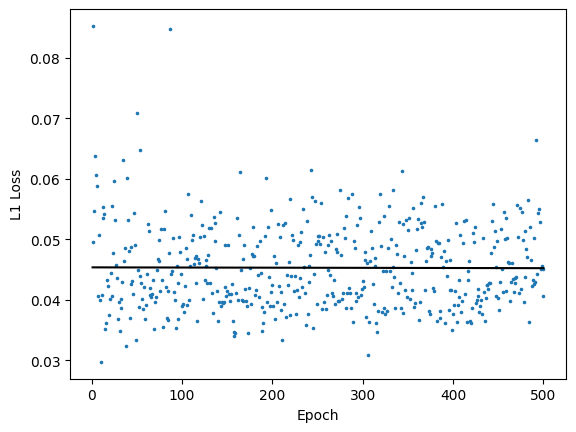
\includegraphics[width=.9\linewidth]{images/l1_loss.png}
\end{center}

\begin{center}
\includegraphics[width=.9\linewidth]{images/ae_loss.png}
\end{center}

AE loss is the spatially discounted reconstruction loss\autocite{zhangVoidFillingBased2020}

\begin{center}
\includegraphics[width=.9\linewidth]{images/ae_loss.png}
\end{center}

\begin{center}
\includegraphics[width=.9\linewidth]{images/wasserstein_loss.png}
\end{center}


\section{Discussion}
\label{sec:orgc56a026}

\section{Conclusion}
\label{sec:orgf6ec5fd}

\section{Future Work}
\label{sec:org91aa311}

\section*{Acknowledgements}

\printbibliography

\section*{Appendices}
\end{document}